\documentclass[a4paper,11pt]{report}
\usepackage{chuan_math_gkt}
\usetikzlibrary{angles,quotes,intersections,patterns,decorations.pathreplacing}
\chuanexamsetup

\begin{document}
\examfontsize

\examsecret{绝密$\bigstar$启用前}

\examtitle{2026年普通高等学校招生全国统一考试（天津卷）}{数\quad 学}

\noticetitle
\begin{examnotice}
\item 答卷前，考生务必将自己的姓名、准考证号填写在答题卡上. 
\item 回答选择题时，选出每小题的答案后，用铅笔把答题卡上对应题目的答案标号涂黑. 如需改动，用橡皮擦干净后，再选涂其他答案标号. 回答非选择题时，将答案写在答题卡上. 写在本试卷上无效. 
\item 考试结束后，将本试卷和答题卡一并交回. 
\end{examnotice}

\examsection{一、选择题：本题共9小题，每小题5分，共45分. 在每小题给出的四个选项中，只有一项符合题目要求.}
\begin{examquestions}
\item 已知全集 $U=\{-2,-1,0,1,2,3\}$，集合 $A=\{-1,0,1,3\}$，集合 $B=\{-2,0,1\}$，则 $(\complement_U A)\cap B=$
\fourchoices{$\{-2\}$}{$\{-2,2\}$}{$\{0,1,2\}$}{$\{-2,0,1,2\}$}

\item 设 $x\in\mathbb R$，则“$x>0$”是“$x^2+3x>0$”的
\twochoices
{充分不必要条件}
{必要不充分条件}
{充要条件}
{既不充分也不必要条件}

\item 为研究候鸟迁徙数量与空气质量指数的关系，在不同空气质量指数 $x$ 下统计候鸟迁徙数量 $y$，得到数据如图所示，其中 $y$ 与 $x$ 的样本相关系数 $r=-0.91$，根据最小二乘法算得 $y=-1.17x+1370.7$，下列说法正确的是

\begin{tightcenter}
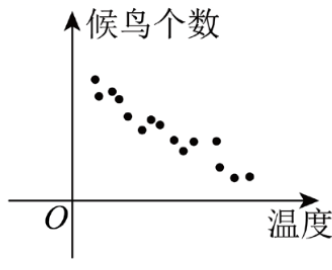
\includegraphics[width=4cm]{figures/2026_tj_q3.png}
\end{tightcenter}

\twochoices
{$y$ 与 $x$ 负相关}
{当 $x=10$ 时，$y$ 一定为 $1359$}
{当 $x=10$ 时，$y$ 一定小于 $1359$}
{两变量无线性关系}

\newpage
\item 函数 $f(x)$ 的部分图象如图所示，则 $f(x)$ 的解析式可能为

\begin{tightcenter}
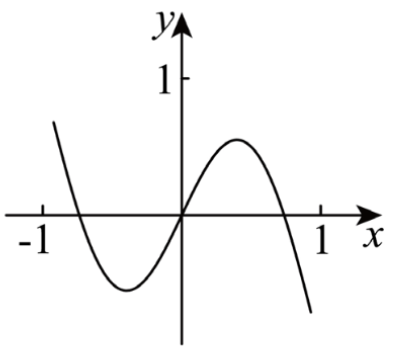
\includegraphics[width=4.0cm]{figures/2026_tj_q4.png}
\end{tightcenter}

\fourchoices
{$x+\sin\pi x$}
{$x-\sin\pi x$}
{$-x+\sin\pi x$}
{$x\cdot\sin\pi x$}

\item 在正方体 $ABCD-A_1B_1C_1D_1$ 中，下列结论错误的是
\twochoices
{$AC\parallel A_1C_1$}
{$CC_1\perp$ 平面 $ABC$}
{平面 $ACD_1\parallel$ 平面 $A_1C_1B$}
{平面 $ADD_1\perp$ 平面 $ACD_1$}

\item 已知函数 $f(x)=|\ln x|$，若 $a=f(2^{0.3})$，$b=f(3^{0.3})$，$c=f(3^{-0.5})$，则 $a,b,c$ 的大小关系为
\fourchoices
{$a<b<c$}
{$b<a<c$}
{$c<b<a$}
{$c<a<b$}

\item 设 $x\neq0$，则 $\left(x+\dfrac1x\right)\left(x+\dfrac4x\right)$ 的最小值为
\fourchoices{$10$}{$9$}{$8$}{$6$}

\item 已知数列 $\{a_n\}$ 的前 $n$ 项和为 $S_n$，$S_{2n}-S_n=n$，$a_3=6$，则 $a_7+a_8=$
\fourchoices{$68$}{$56$}{$-3$}{$-4$}

\item 已知双曲线 $\dfrac{x^2}{a^2}-\dfrac{y^2}{b^2}=1(a>0,b>0)$ 的左焦点为 $F$，$A$ 是右顶点，$P$ 是双曲线上一点，满足 $|FA|=|FP|$，$\angle FAP=30^\circ$，则双曲线的离心率为
\fourchoices
{$4$}
{\tallchoice{$\dfrac83$}}
{\tallchoice{$\dfrac85$}}
{\tallchoice{$\dfrac43$}}
\end{examquestions}

\examsection{二、填空题：本题共6小题，每小题5分，共30分.}
\begin{examquestions}[start=10]
\item 已知 $\mathrm{i}$ 是虚数单位，化简 $(3+\mathrm{i})^2=$ \blank.

\item 在 $(x+2y)^4$ 的展开式中，$x^3y$ 的系数为 \blank.

\item 在 $\triangle ABC$ 中，$BC=4$，$AC=3$，$\cos A=-\dfrac14$，则 $\sin B=$ \blank.

\item 箱子中有一个红球，两个黄球，三个白球. 有放回地取三次，每次取一个，三次都没取到黄球的概率是 \blank；在三次都没取到黄球的条件下，至少取到一次红球的概率是 \blank.

\item 已知 $|\vec a|=\vec a\cdot\vec b=1$，$|\vec b|>1$，记 $\vec c=\lambda\vec a+\mu\vec b$. 当 $\vec a+\vec b-\vec c=\vec0$ 时，$\lambda+\mu=$ \blank；当 $|\vec a+\vec b-\vec c|=1$ 时，$\lambda+\mu$ 的取值范围是 \blank.

\item 在平面内，$O$ 为坐标原点，抛物线 $y^2=2x$ 上有 $A,B,C,D$ 四个点，$A,B,C,D$ 的纵坐标分别为 $y_A,y_B,y_C,y_D$，直线 $AB$ 与直线 $CD$ 交 $x$ 轴于点 $P$，直线 $AC$ 交 $x$ 轴于点 $M$，直线 $BD$ 交 $x$ 轴于点 $N$. 以下说法正确的有 \blank.

\gktcircled{1} 若 $M$ 与抛物线焦点重合，则 $y_Ay_C=-2$；

\gktcircled{2} $y_Ay_B=y_Cy_D$；

\gktcircled{3} $|OM|\cdot|ON|=2|OP|^2$；

\gktcircled{4} $|y_A-y_C|\cdot|OP|=|y_B-y_D|\cdot|OM|$；

\gktcircled{5} $\dfrac{S_{\triangle ACP}}{S_{\triangle BDP}}=\left(\dfrac{|OM|}{|ON|}\right)^2$.
\end{examquestions}

\examsection{四、解答题：本题共5小题，共75分. 解答应写出文字说明、证明过程或演算步骤.}
\begin{examanswers}[start=16]
\item（14分）

已知函数 $f(x)=\sin\left(2x+\dfrac{\pi}{6}\right)$.

\subq{（1）}{求 $f(x)$ 的最小正周期；}

\subq{（2）}{若 $x\in\left[-\dfrac{\pi}{6},\dfrac{\pi}{12}\right]$，求 $f(x)$ 的最大值和最小值；}

\subq{（3）}{若 $\alpha\in\left(0,\dfrac{\pi}{2}\right)$，$\sin\alpha=\dfrac{\sqrt3}{3}$，求 $f(\alpha)$.}

\item（15分）

在长方体 $ABCD-A_1B_1C_1D_1$ 中，$AB=2$，$AA_1=3$，$AD=4$，$A_1E=3ED_1$，$C_1F=2FC$.

\noindent\begin{minipage}[t]{0.60\linewidth}
\subq{（1）}{求证：$BD\perp$ 平面 $CEF$；}

\subq{（2）}{求平面 $AEF$ 与平面 $CEF$ 的夹角的余弦值；}

\subq{（3）}{求三棱锥 $A-CEF$ 的体积.}
\end{minipage}\hfill
\begin{minipage}[t]{0.27\linewidth}
\vspace{-1.0em}
\centering
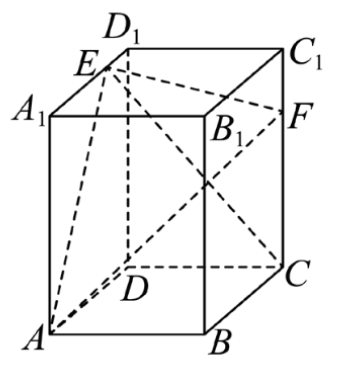
\includegraphics[width=\linewidth]{figures/2026_tj_q17.png}
\end{minipage}
\vspace{-2em}
\item（15分）

已知椭圆 $C:\dfrac{x^2}{a^2}+\dfrac{y^2}{b^2}=1(a>b>0)$ 的离心率为 $\dfrac12$，椭圆被直线 $x=b$ 截得的线段长为 $\sqrt3$.

\subq{（1）}{求 $C$ 的标准方程；}

\subq{（2）}{斜率为 $-\sqrt3$ 的直线与圆 $x^2+y^2=b^2$ 相切，且该直线交椭圆于 $P(x_1,y_1)$，$Q(x_2,y_2)(y_1<y_2)$，$A$ 是椭圆的上顶点. 记 $AP,AQ$ 的斜率分别为 $k_1,k_2$，求 $\dfrac{k_1}{k_2}$ 的值.}

\item（15分）

等差数列 $\{a_n\}$ 与等比数列 $\{b_n\}$ 满足：$a_1=2$，$b_1=1$，$a_2=b_1+b_2$，$a_4=b_3-b_1$.

\subq{（1）}{求数列 $\{a_n\},\{b_n\}$ 的通项公式；}

\subq{（2）}{记 $E_n=\{x\in\mathbb R\mid x\leq n,\exists k\in\mathbb N^*\text{ 使得 }x=a_k\text{ 或 }x=b_k\}$，$c_n$ 为 $E_n$ 中的元素个数.}

\subq{（i）}{求 $c_{3^n}$；}

\subq{（ii）}{求 $\displaystyle\sum_{m=1}^{3^n-1}(-1)^m\cdot a_m\cdot c_m$.}

\item（16分）

已知 $f(x)=e^x-\dfrac23\sin x$.

\subq{（1）}{求 $f(x)$ 在点 $(0,f(0))$ 处的切线方程；}

\subq{（2）}{当 $x\in\left[-\dfrac13,+\infty\right)$ 时，证明：$f(x)\geq1+\dfrac{x}{3}$；}

\subq{（3）}{$\forall n\in\mathbb N^*$，$f(1)\cdot f\left(\dfrac12\right)\cdot f\left(\dfrac13\right)\cdots f\left(\dfrac1n\right)\geq(n+1)^a$ 恒成立，求实数 $a$ 的最大值.}
\end{examanswers}

\end{document}